	
	
	В одном взятом сэмпле обычно находится 16 бит. Это означает, что у нас $2^{16}$ значений. Нам приходится делать softmax на $2^{16}$ значений. Очень много получается, хотим сделать поменьше. 
	
	Рассматриваемый метод позволяет ужать значения амплитуд, сохранив по максимуму первоначальную информацию. 
	
	Интуиция: человеческое ухо слышит в лог шкале: мы хорошо различаем звуки при низких амплитудах и плохо различаем при высоких. Нам надо хранить низкие амплитуды в высоком разрешении, а высокие амплитуды в низком, ибо мы и так их особо не слышим. 
	
	Реализация идеи хороша видна на следующем графике \ref{fig:12_plot}: здесь показано, как звуки с разными амплитудами преобразуются согласно данному кодированию 
	
	
		\begin{figure}[H]
\centering
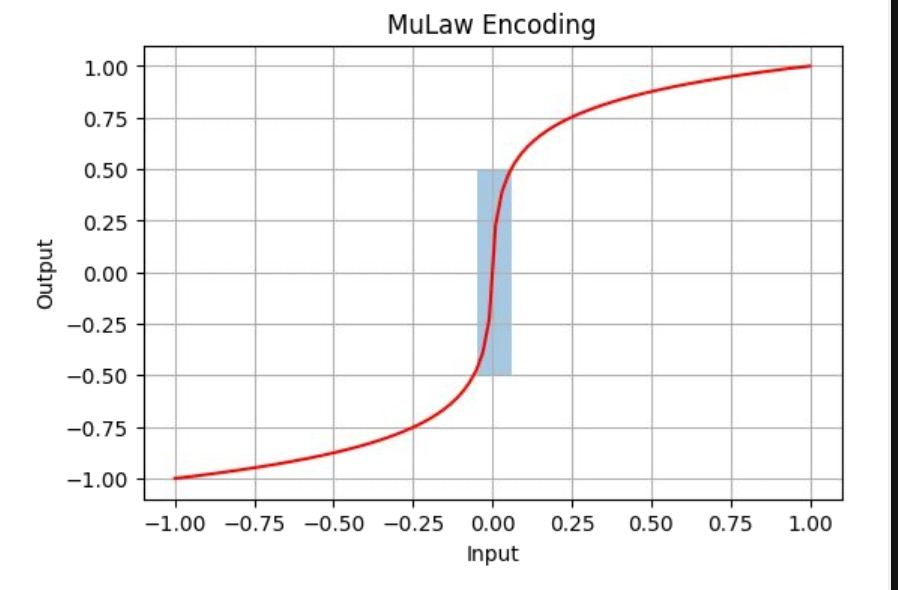
\includegraphics[width=0.7\linewidth]{12_trans.jpg}
\caption{Визуализация Mu law Encoding}
\label{fig:12_plot}
\end{figure}

Как можно увидеть, от -0.1 до 0.1 мы очень компактно храним входные частоты, но чем дальше амплитуда, тем больше у нас становится шаг(скорость функции возрастае), и соответственно в тем меньшем разрешении мы храним звуки с указанной амплитудой. 

Гиперпараметром считается количество конечных значений, в которые мы хотим перевести все наши амплитуды. 


Формула:

\begin{equation}
	    f(x_t) = \text{sign}(x_t) \dfrac{\ln(1+\mu|x_t|)}{\ln(1+\mu)}
	    \label{eq:12_formula}
\end{equation}
	
$\mu$ - это просто параметр сжатия ( обычно он вот такой - 255). 

x- нормализованное число, которое подвергается сжатию. 
